\documentclass[11pt]{article}
\usepackage[margin=1in]{geometry}
\usepackage{array}
\usepackage{enumitem}
\usepackage{times}
\usepackage{graphicx}

\setlength{\parindent}{0pt}
\setlength{\parskip}{6pt}
\renewcommand{\arraystretch}{1.25}

\newcommand{\guil}[1]{\textless\textless #1\textgreater\textgreater}

\begin{document}

\begin{center}
{\LARGE \textbf{Hyperlocal Courier Dispatch \& Tracking Engine}}\\[4pt]
{\large Lab 3 -- Component Modelling \& Architectural Pattern Selection}\\[2pt]
\end{center}

\vspace{4pt}

\section*{1. Scenario Review}

The system is an on-demand parcel delivery platform. A sender client creates a courier request, the system matches it to the nearest active rider within a 3~km radius, generates optimal multi-stop routes for riders carrying several parcels, streams live GPS location back to the sender, and enforces OTP verification at the destination before a delivery is marked complete.

Key functional needs (from Lab 1): request creation (FR-002), nearest-rider matching (FR-001), rider accept/view requests (FR-003), multi-stop routing (FR-004), and OTP verification at handover (FR-005). Key non-functional needs: live telemetry to the sender with under 2-second latency (NFR-001) and 99.9\% uptime during peak hours (NFR-002).

Main challenges:
\begin{itemize}[leftmargin=1.4em,nosep]
\item \textbf{Performance:} high-frequency GPS telemetry must reach senders in under 2 seconds even at peak load, while matching and routing are computationally heavier but less frequent.
\item \textbf{Reliability:} a fault in one feature (e.g.\ routing) must not bring down tracking or OTP verification, since uptime targets are strict.
\item \textbf{Security:} OTP handover and rider/sender data must be protected, and verification logic kept isolated to prevent fraud.
\end{itemize}

\section*{2. Architectural Style Analysis}

Each candidate style was assessed against the requirements above.

\begin{tabular}{|p{2.6cm}|p{5.0cm}|p{5.4cm}|}
\hline
\textbf{Style} & \textbf{Fit for this scenario} & \textbf{Main drawback here} \\
\hline
Layered & Clear separation of concerns; simple to reason about. & All features scale together; a single deployment unit makes it hard to scale telemetry independently or isolate faults. \\
\hline
Client--Server & Simple deployment; easy data consistency for a single central server. & The central server is a single point of failure and a scalability bottleneck, which conflicts with the 99.9\% uptime and peak-load latency targets. \\
\hline
Microservices & Independent scaling and deployment per feature; fault isolation; supports a dedicated high-throughput telemetry path. & More operational complexity and network latency between services; needs care with data consistency. \\
\hline
\end{tabular}

\section*{3. Architecture Selection \& Component Identification}

\textbf{Selected architecture: Microservices.} The workload has features with very different load profiles (constant GPS telemetry vs.\ bursty matching and routing), a strict latency target on one path, and a high uptime requirement. Microservices let each concern scale and fail independently, which the other two styles cannot do well.

The following components were identified for the chosen architecture:

\begin{tabular}{|p{4.3cm}|p{7.2cm}|p{1.6cm}|}
\hline
\textbf{Component} & \textbf{Responsibility} & \textbf{Req.} \\
\hline
Sender Client App & Touch/mobile UI to create requests and view live tracking. & FR-002, NFR-001 \\
\hline
Rider Client App & Rider UI to view/accept requests, follow routes, enter OTP. & FR-003, FR-005 \\
\hline
API Gateway & Single entry point; authentication, TLS, request routing. & -- \\
\hline
Dispatch Service & Creates/manages requests and matches the nearest rider; orchestrates the other services. & FR-001, FR-002 \\
\hline
Routing Service & Generates optimal multi-stop routes for a rider. & FR-004 \\
\hline
Tracking Service & Ingests rider GPS telemetry and streams it to senders. & NFR-001 \\
\hline
OTP Verification Service & Issues and validates delivery OTPs at handover. & FR-005 \\
\hline
Database & Persists requests, riders, routes and OTP records. & -- \\
\hline
\end{tabular}



\section*{4. Component Diagram}

The UML component diagram uses \guil{component} notation, provided interfaces (ball) on each service and required interfaces (socket) on each consumer, connected as assembly connectors.

\begin{figure}[ht]
\centering
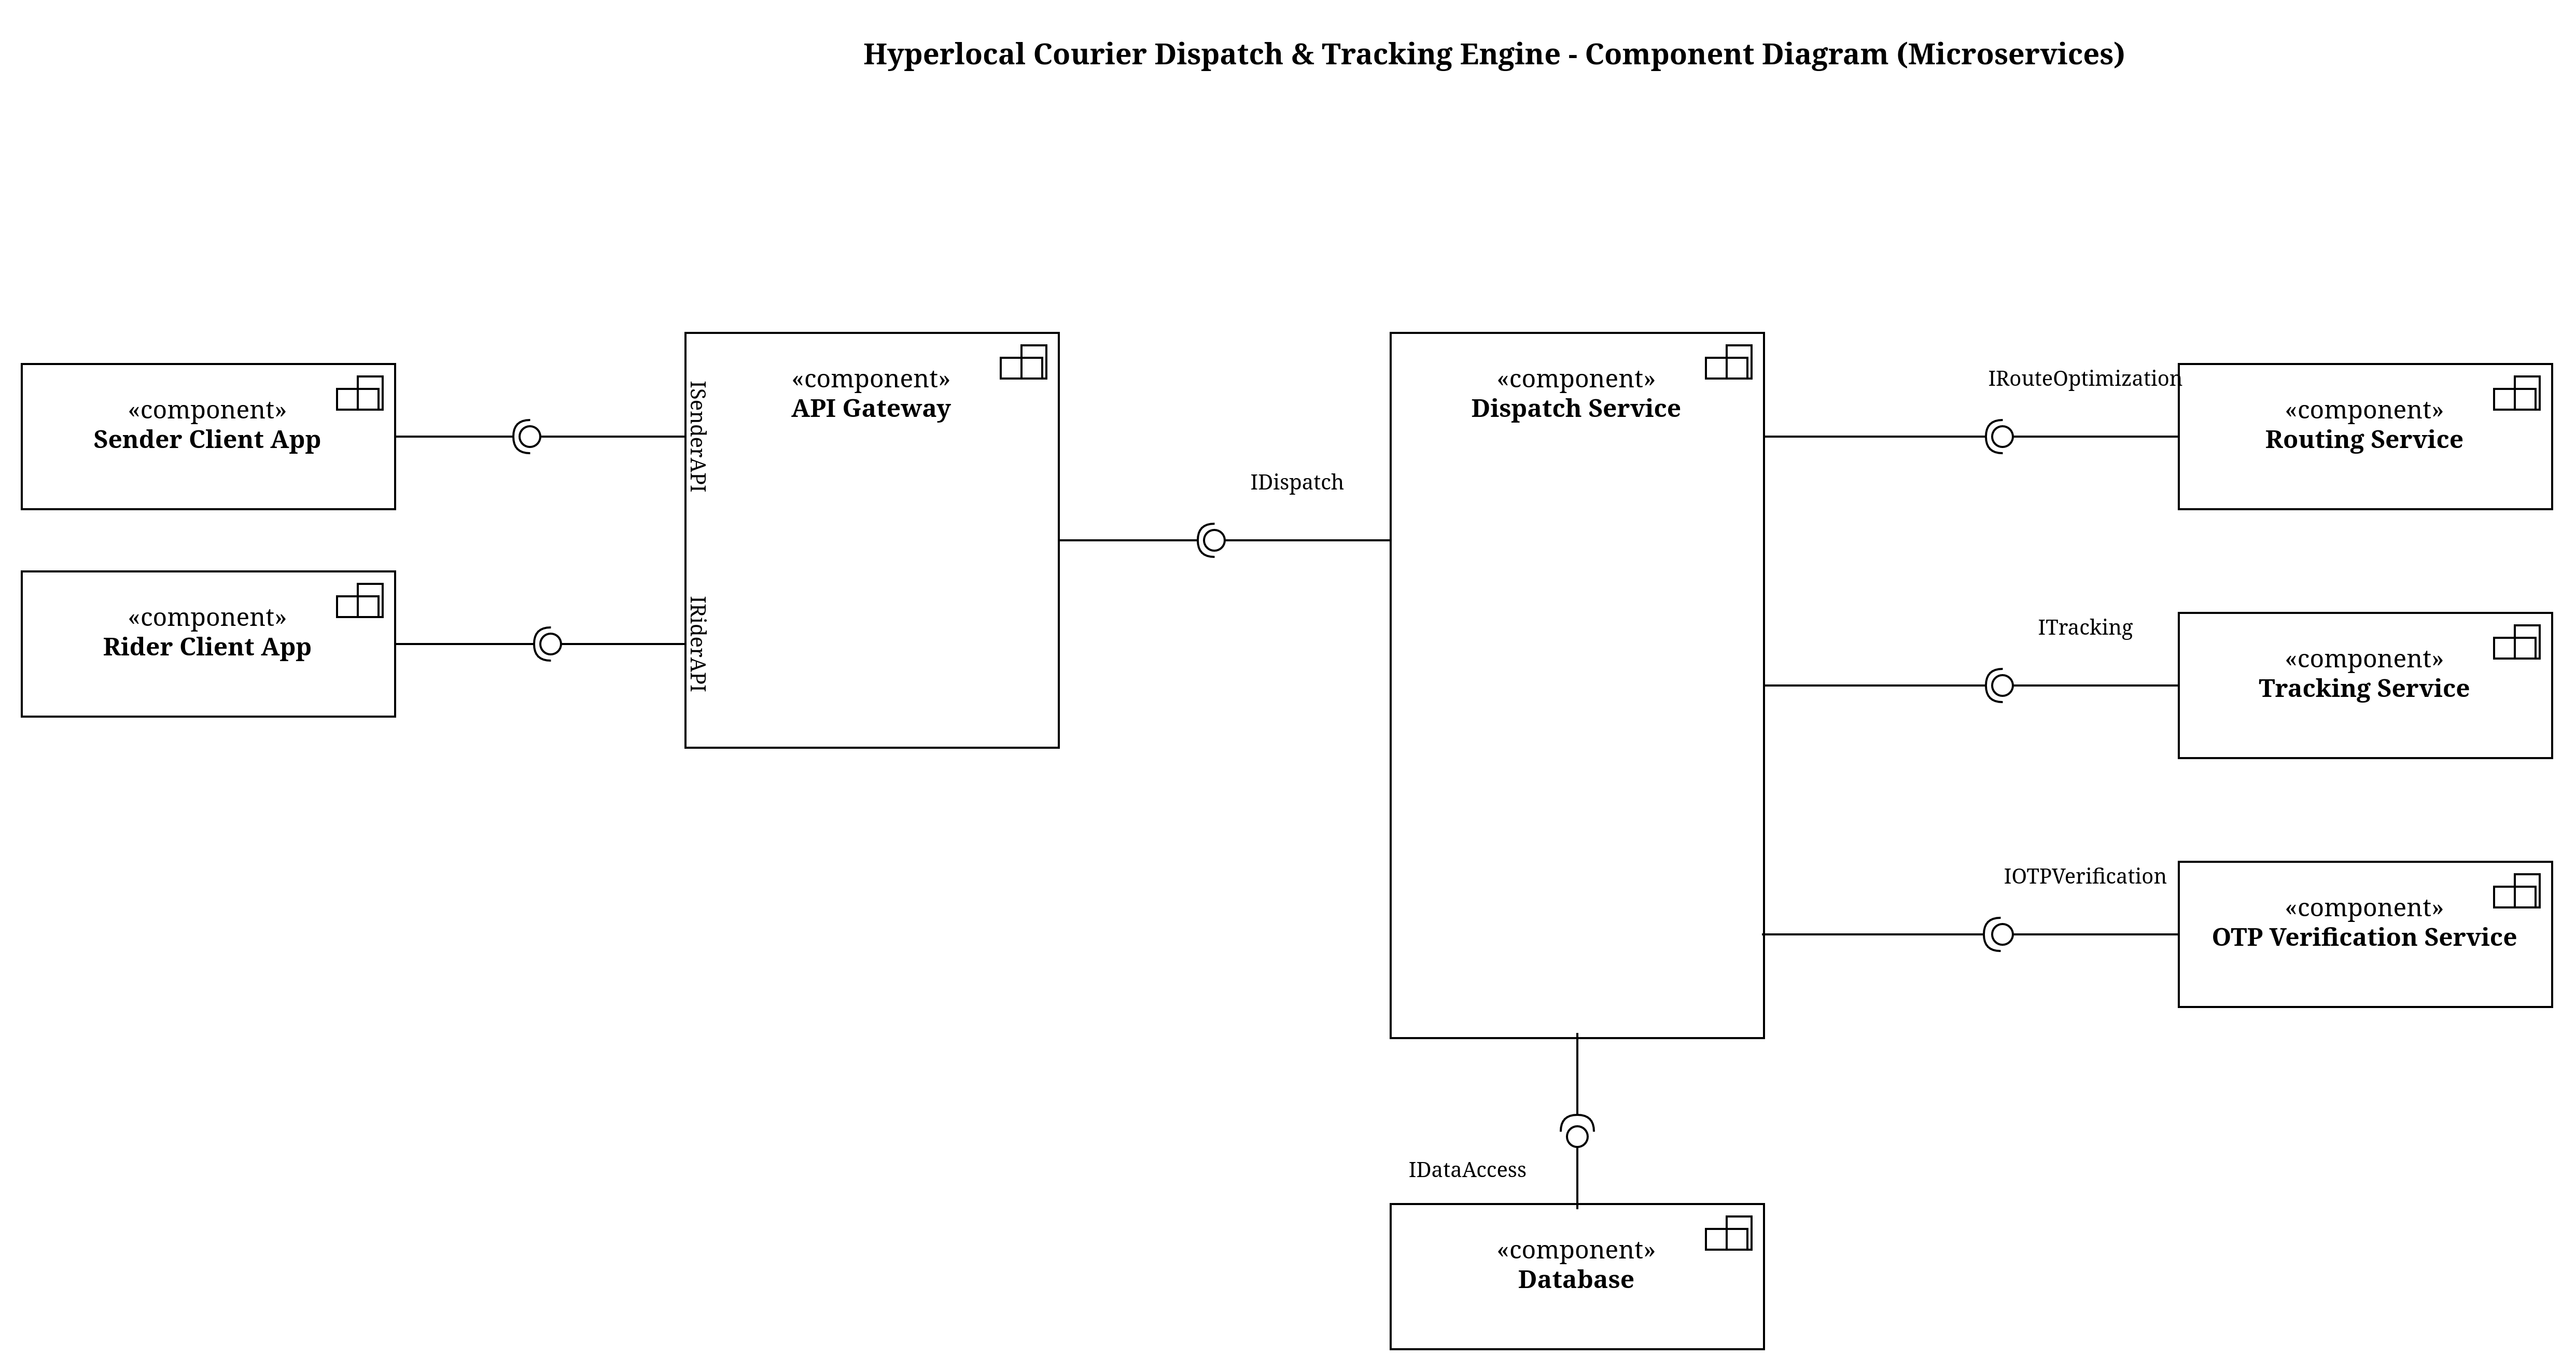
\includegraphics[width=\textwidth]{component_diagram.png}
\caption{Component diagram for the Hyperlocal Courier Dispatch \& Tracking Engine.}
\end{figure}

Interfaces shown between components:

\begin{tabular}{|p{3.3cm}|p{2.7cm}|p{2.9cm}|p{3.4cm}|}
\hline
\textbf{Interface} & \textbf{Provided by} & \textbf{Required by} & \textbf{Protocol} \\
\hline
ISenderAPI & API Gateway & Sender Client App & HTTPS / REST \\
\hline
IRiderAPI & API Gateway & Rider Client App & HTTPS / REST \\
\hline
IDispatch & Dispatch Service & API Gateway & REST \\
\hline
IRouteOptimization & Routing Service & Dispatch Service & REST \\
\hline
ITracking & Tracking Service & Dispatch Service & WebSocket / stream \\
\hline
IOTPVerification & OTP Verification Service & Dispatch Service & REST \\
\hline
IDataAccess & Database & Dispatch Service & SQL \\
\hline
\end{tabular}



\section*{5. Written Justification}

\textbf{Architecture Selection:} I chose a Microservices architecture for the Hyperlocal Courier Dispatch \& Tracking Engine.

\textbf{Architectural choice.} The system is decomposed into independently deployable services (Dispatch, Routing, Tracking, OTP Verification) behind an API Gateway, each owning a single responsibility and communicating over well-defined interfaces.

\textbf{Two reasons.}
\begin{enumerate}[leftmargin=1.5em,nosep]
\item \emph{Different load profiles need independent scaling.} Live GPS telemetry is continuous and high-volume, whereas matching and route optimisation are heavier but bursty. As separate services, the Tracking Service can be scaled out on its own to sustain the under-2-second latency target (NFR-001) without over-provisioning the whole system.
\item \emph{Fault isolation supports the uptime target.} If the Routing Service degrades, the Tracking and OTP Verification services keep running, so senders still see live status and deliveries can still be completed. This containment of failures directly helps meet the 99.9\% uptime requirement (NFR-002), which a single-server design cannot guarantee.
\end{enumerate}

\textbf{Security advantage.} All external traffic passes through the API Gateway, which centralises authentication and TLS termination, so services are not exposed directly. OTP verification runs as its own isolated service, keeping the verification logic and stored OTPs compartmentalised; a compromise in another service does not expose them, and the blast radius of any breach is limited to a single service.

\textbf{Performance benefit.} Because the Tracking Service is independent, it can be scaled horizontally and tuned (streaming transport, dedicated instances) to keep GPS updates under the 2-second latency target during peak load, without a monolithic bottleneck slowing the matching or routing paths.

\end{document}
